%>>>>>>>>>>>>>>>>>>>>>>>>>> ПЕРЕМЕННЫЕ >>>>>>>>>>>>>>>>>>>>>>>>>>>>>>>>>>>
%>>>>> Информация о кафедре
%\newcommand{\year}{2021 г.}  % Год устанавливается автоматически
\newcommand{\city}{Санкт-Петербург}  %  Футер, нижний колонтитул на титульном листе
\newcommand{\university}{Национальный исследовательский университет ИТМО}  % первая строка
\newcommand{\department}{Факультет программной инженерии и компьютерной техники}  % Вторая строка
\newcommand{\major}{Направление программная инженерия}  % Треьтя строка
% Пусть будет. Проще закоментить лишнее.
\newcommand{\education}{Образовательная программа системное и прикладное программное обеспечение}  % четвертая строка
%\newcommand{\specialization}{}  % пятая строка

%<<<<< Информация о кафедре

%>>>>> Назание работы
\newcommand{\reporttype}{ОТЧЕТ ПО ЛАБОРАТОРНОЙ РАБОТЕ} % тип работы, (главный заголовок титульного листа)
\newcommand{\lab}{Лабораторная работа}          % вид работы
\newcommand{\labnumber}{№ 1}                    % порядковый номер работы
\newcommand{\subject}{Основы профессиональной деятельности}         % учебный предмет
% \newcommand{\labtheme}{Принципы ООП}            % Тема лабораторной работы
\newcommand{\variant}{№ 1402}                % номер варианта работы

\newcommand{\student}{Бых Даниил Максимович}    % определение ФИО студента
\newcommand{\studygroup}{P3109}                 % определение учебной группы
\newcommand{\teacher}{% принимающий
    Деменев Т. Г.% ФИО практика
}
%<<<<<<<<<<<<<<<<<<<<<<<<<< ПЕРЕМЕННЫЕ <<<<<<<<<<<<<<<<<<<<<<<<<<<<<<<<<<<


%>>>>>>>>>>>>>>>>>>>>>> ПРЕАМБУЛА >>>>>>>>>>>>>>>>>>>>>>>>>
\documentclass[14pt,final,oneside]{extreport}% класс документа, характеристики
%>>>>> Разметка документа
\usepackage[a4paper, mag=1000, left=3cm, right=1.5cm, top=2cm, bottom=2cm, headsep=0.7cm, footskip=1cm]{geometry} % По ГОСТу: left>=3cm, right=1cm, top=2cm, bottom=2cm,
\linespread{1} % межстройчный интервал по ГОСТу := 1.5
%<<<<< Разметка документа

\setlength{\parindent}{1.25cm}

%>>>>> babel c языковым пакетом НЕ должны быть первым импортируемым пакетом
\usepackage[utf8]{inputenc}
\usepackage[T1,T2A]{fontenc}
\usepackage[russian]{babel}
% \usepackage{lmodern}
%<<<<<

%\usepackage{cmap} %поиск в pdf

%>>>...>> прочие полезные пакеты
\usepackage{amsmath,amsthm,amssymb}
\usepackage{mathtext}
\usepackage{braket}
\usepackage{indentfirst}
\usepackage{graphicx}
\usepackage{float}
\usepackage{changepage}
\graphicspath{{assets}}
\DeclareGraphicsExtensions{.pdf,.png,.jpg}
%\usepackage{bookmark}

\usepackage[dvipsnames]{xcolor}
\usepackage{hyperref}  % Использование ссылок
\hypersetup{%  % Настройка разметки ссылок
    colorlinks=true,
    linkcolor=blue,
    filecolor=magenta,
    urlcolor=magenta,
%pdftitle={Overleaf Example},
%pdfpagemode=FullScreen,
}

\usepackage{diagbox}
\usepackage[letterspace=150]{microtype} % Спэйсинг (межбуквенный интервал для саголовка) \lsstyle
% \usepackage{csvsimple} %импорт содержимого таблицы из csv

%>>> верстка в 2 колонки
\usepackage{multicol} % многоколоночная верстка
\setlength{\columnsep}{.15\textwidth} % определение ширины разделителя между колонками

\usepackage{tikz} % пакет для векторной графики, чтобы рисовать красивый разделитель колонок

%>>>>> Использование листингов
\usepackage{listings}
\usepackage{caption}
\DeclareCaptionFont{white}{\color{white}}
\DeclareCaptionFormat{listing}{\colorbox{gray}{\parbox{\textwidth}{#1#2#3}}}

\captionsetup[lstlisting]{format=listing,labelfont=white,textfont=white} % Настройка вида описаний
\lstset{  % Настройки вида листинга
    inputencoding=utf8, extendedchars=\true, keepspaces = true, % поддержка кириллицы и пробелов в комментариях
    language={},            % выбор языка для подсветки (здесь это Pascal)
    basicstyle=\small\sffamily, % размер и начертание шрифта для подсветки кода
    numbers=left,               % где поставить нумерацию строк (слева\справа)
    numberstyle=\tiny,          % размер шрифта для номеров строк
    stepnumber=1,               % размер шага между двумя номерами строк
    numbersep=5pt,              % как далеко отстоят номера строк от подсвечиваемого кода
    backgroundcolor=\color{white}, % цвет фона подсветки - используем \usepackage{color}
    showspaces=false,           % показывать или нет пробелы специальными отступами
    showstringspaces=false,     % показывать илигнет пробелы в строках
    showtabs=false,             % показывать или нет табуляцию в строках
    frame=single,               % рисовать рамку вокруг кода
    tabsize=2,                  % размер табуляции по умолчанию равен 2 пробелам
    captionpos=t,               % позиция заголовка вверху [t] или внизу [b]
    breaklines=true,            % автоматически переносить строки (да\нет)
    breakatwhitespace=false,    % переносить строки только если есть пробел
    escapeinside={\%*}{*)}      % если нужно добавить комментарии в коде
}

\definecolor{codegreen}{rgb}{0,0.6,0}
\definecolor{codegray}{rgb}{0.5,0.5,0.5}
\definecolor{codepurple}{rgb}{0.58,0,0.82}
\definecolor{backcolour}{rgb}{0.95,0.95,0.92}

\lstdefinestyle{mystyle}{
backgroundcolor=\color{backcolour},
commentstyle=\color{codegreen},
keywordstyle=\color{magenta},
numberstyle=\tiny\color{codegray},
stringstyle=\color{codepurple},
basicstyle=\ttfamily\footnotesize,
breakatwhitespace=false,
breaklines=true,
captionpos=b,
keepspaces=true,
numbers=left,
numbersep=5pt,
showspaces=false,
showstringspaces=false,
showtabs=false,
tabsize=2
}
\lstset{style=mystyle}
%<<<<< Использование листингов


\sloppy % Решение проблем с переносами (с. 119 книга Львовского)
\emergencystretch=25pt


%>>>>>>>>>>>>>>>> ДОПОЛНИТЕЛЬНЫЕ КОМАНДЫ {Для соответствия ГОСТ} >>>>>>>>>>>>>>
%>>>>>> математические функции для удобства
\newcommand{\tx}{\text}
\newcommand{\eps}{\varepsilon}
\renewcommand{\phi}{\varphi}
\newcommand{\limit}{\displaystyle\lim}
\newcommand{\oo}{\infty}
\newcommand{\De}{\Delta}
\newcommand{\cd}{\cdot}
\newcommand{\df}{\partial}
\newcommand{\ndash}{\textendash}
\newcommand{\mdash}{\textemdash}

%>>>>> Аннотирование
\newcommand{\note}[2]{\overbrace{#1}^{#2}}% скобка сверху для комментария
% \overset{}{}% для указания символа над другим смиволом
% \underset{}{}% для указания символа под другим смиволом
%<<<<< Аннотирование

%>>>>>> Матрицы
\DeclareMathOperator{\rank}{rank}
\newcommand{\tvec}[1]{\mathbfit{#1}}% "text vector"
\newcommand{\mtx}[1]{\mathrm{#1}}
\newcommand{\transposed}[1]{{#1}^{\mathrm{T}}}
%>>>>>> Матрицы

%>>>>> Скобки
\newcommand{\lt}{\left}
\newcommand{\rt}{\right}
\newcommand{\la}{\langle}% '<'
\newcommand{\ra}{\rangle}% '>'
\newcommand{\avg}[1]{\langle{#1}\rangle}% '<X>'
%<<<<< Скобки

%>>>>> Дроби
\newcommand{\cf}[2]{\cfrac{#1}{#2}}
\newcommand{\fr}[2]{\frac{#1}{#2}}
%<<<<< Дроби


%>>>>> Стрелки
\newcommand{\Rarr}{\Rightarrow}% ⇒ следствие | лучше использовать \implies
\newcommand{\LRarr}{\Leftrightarrow}% равносильно | лучше  использовать \iff
\newcommand{\rarr}{\xrightarrow{}}% → стрелка вправо
\newcommand{\nwarr}{\nwarrow}% ↖ север-запад стрелка
\newcommand{\nearr}{\nearrow}% ↗ север-восток стрелка
\newcommand{\swarr}{\swarrow}% ↙ юг-запад стрелка
\newcommand{\searr}{\searrow}% ↘ юг-восток стрелка

\newcommand{\raises}{\nwarrow}% возрастает
\newcommand{\increases}{\nwarrow}% возрастает
\newcommand{\falls}{\swarrow}% убывает
\newcommand{\decreases}{\swarrow}% убывает

%{{{
\makeatletter
\newcommand{\impliesby}[2][]{\ext@arrow 0359\Leftrightarrowfill@{#1}{#2}}% следствие с надписью
\makeatother
%}}}

%{{{
\makeatletter
\newcommand{\iffby}[2][]{\ext@arrow 0359\Rightarrowfill@{#1}{#2}}% равносильность с надписью
\makeatother
%}}}
%<<<<< Стрелки

% Функции для удобного описания формул: https://tex.stackexchange.com/questions/95838/how-to-write-a-perfect-equation-parameters-description


%<<<<<< математические функции для удобства
%>>>>>> Стиль текста
\newcommand{\hex}[1]{\texttt{0{\footnotesize{x}}#1}}
\newcommand{\ttt}[1]{\texttt{#1}}
%<<<<<< Стиль текста

\newcommand\Chapter[3]{%
% Принимает 3 аргумента - название главы и дополнительный заголовок и множитель ширины загловка (можно ничего)
\refstepcounter{chapter}%
\chapter*{%
%\hfill % заполнение отступом пространства до заголовка
\begin{minipage}{#3\textwidth} % Можно изменить ширину министраницы (заголовка)
\flushleft % Выранивание заголовка по левому краю параграфа (заголовка)
%\flushright % Выранивание заголовка по правому краю параграфа (заголовка)
\begin{huge}%
% Отключена нумерация глав в тексте:
% \textbf{\chaptername\ \arabic{chapter}\\}
\textbf{#1}% Первый заголовок
\end{huge}%
\\% Перенос сторки
\begin{Huge}
#2% Второй заголовок
\end{Huge}
\end{minipage}
}%
% Отключена нумерация для chapter в toc (table of contents), т.е. Оглавлении (Содержании):
% \addcontentsline{toc}{chapter}{\arabic{chapter}. #1}
% Представление главы в содержании:
\addcontentsline{toc}{chapter}{#1. #2}%
}

\newcommand\Section[1]{
% Принимает 1 аргумент - название секции
\refstepcounter{section}
\section*{%
\raggedright
% Отключена дополнительная нумерация chapter в section в тексте документа:
% \arabic{chapter}.\arabic{section}. #1}
% Отключена любая нумарация section в тексте документа:
\arabic{section}. #1%
}

% Отключена дополнительная нумерация chapter в section в toc (table of contents) Оглавлении (Содержании):
% \addcontentsline{toc}{section}{\arabic{chapter}.\arabic{section}. #1}
\addcontentsline{toc}{section}{\arabic{section}. #1}
}


\newcommand\Subsection[1]{
% Принимает 1 аргумент - название подсекции
\refstepcounter{subsection}
\subsection*{%
\raggedright%
% Отключена дополнительная нумерация chapter в section в тексте документа (можно добавить отступ с помощью \hspace*{12pt}):
% \arabic{chapter}.\arabic{section}.\arabic{subsection}. #1}
\arabic{section}. \arabic{subsection}. #1
}
% Отключена дополнительная нумерация chapter в section в Оглавлении (Содержании):
%\addcontentsline{toc}{subsection}{\arabic{chapter}.\arabic{section}.\arabic{subsection}. #1}
\addcontentsline{toc}{subsection}{\arabic{subsection}. #1}
}


\newcommand\Figure[4]{
% Принимает 4 аргумента - название файла изображения, ее размер в тексте, описание, лэйбл (псевдоним в формате "fig:name")
%
\refstepcounter{figure}
\begin{figure}[H] %- \usepackage {float} %[h]
\begin{center}
\fbox{
\includegraphics[width=#2]{#1}
}
\end{center}
\begin{center}
Рис.~\arabic{figure}. #3.
\end{center}
%\caption{#3}
\label{fig:#4}
\end{figure}
}


\newcommand\Table[3]{
% Принимает 3 аргумента --- лэйбл name(#1) (псевдоним в формате "tab:name"), ее описание(#2), содержание таблицы(#3)
% ВАЖНО!: от этого способа страдает нумерация описаний, можно использовать создание таблиц через googlesheet
%
\renewcommand{\arraystretch}{1.2} % Установка высоты строки таблицы по умолчанию, увеличенное на 0.2 пункта
% \refstepcounter{table}% увеличение счетчика таблиц
\begin{table}[Htpb]% "right Here", "top", "new page", "bottom"
\label{tab:#1}% лэйбл таблицы, для ссылок
\resizebox{\columnwidth}{!}{% сжимает очень широкие таблицы, чтобы вместить на страницу
#3% Содержимое таблицы
}
%
\caption{#2}% Описание стандартными средствами для используемого окружения (table)
% \captionof{table}{#2}% Описание стандартными средствами
% \captionof*{figure}{\flushleft \textsc\textbf{Рис. 1.}}% Описание стандартными средствами, как рисунка
%
%%> кастомное описание
% \begin{flushleft}% Кастомное описание
%     % \textsf{%
%         \textbf{%
%             \\[2mm]
%             #2% Описание к картинке
%         }%
%         % \\[8mm]% Отступ
%     % }%
% \end{flushleft}
%%< кастомное описание
\end{table}
\renewcommand{\arraystretch}{1} % возврат установка высоты строки таблицы по умолчанию на 1
}


\newcommand\CustomFigure[4]{ % multicols не умеют в table и figure, поэтому приходится извращаться % вставка таблицы с меткой рисунка
% Принимает 4 аргумента - название файла изображения, ее размер в тексте, описание, лэйбл (псевдоним в формате "fig:name")
%
\refstepcounter{figure}
\begin{figure}[ht]% "here", "top"
\begin{center}
\includegraphics[width=#2]{#1}
\end{center}
%
%\caption{#3}
\captionof{figure}{#3}% описание стандартными средствами
% \begin{center}
\begin{flushleft} % Кастомное описание
\textbf{%
#3% Текст описания
}
\end{flushleft}
% \end{center}
%
\label{fig:#4}% Лэйбл, для ссылок
\end{figure}
}


\newcommand\CustomTableFigure[3]{% multicols не умеют в table и figure, поэтому приходится извращаться % вставка таблицы с меткой рисунка
%
% Принимает 3 аргумента --- лэйбл name(#1) (псевдоним в формате "tab:name"), ее описание(#2), содержание таблицы(#3)
%
\begin{center}
\refstepcounter{figure}
\label{tab:#1}% лэйбл таблицы, для ссылок
\resizebox{\columnwidth}{!}{% сжимает очень широкие таблицы, чтобы вместить на страницу
#3% Содержание таблицы
}
%
\captionof{figure}{#2}% Описание стандартными средствами
% \captionof*{figure}{\flushleft \textsc\textbf{Рис. 1.}}% Описание стандартными средствами
%
\begin{flushleft}% Кастомное описание
% \textsf{%
\textbf{%
\\[2mm]
#2% Описание к картинке
}%
% \\[8mm]% Отступ
% }%
\end{flushleft}
\end{center}
}


\newcommand{\InkscapeFigure}[4]{% Вставки иллюстраций из Inkscape (pdf+latex)
%
% Принимает 4 параметра: #1 название файла, #2 описание, #3 лейбл #4 размер
%
% \begin{minipage}{#4}
\begin{figure}[htbp]
\centering
\def\svgwidth{#4}
\import{./figures/}{#1.pdf_tex}
\caption{#2}
\label{fig:#3}
\end{figure}
% \end{minipage}
}


\newcommand\Equation[3]{% Кастомное оформление выражений
%
% Принимает 3 аргумента --- лэйбл name (#1) (псевдоним в формате "tab:name"), его описание(#2), содержание выражения (#3)
%
\textbf{#2}% описание
\begin{equation}
#3% содержимое выражений
\label{eq:#1}% лэйбл
\end{equation}
}

%<<<<<<<<<<<<<<<<<<<<<<<<<<<< ДОПОЛНИТЕЛЬНЫЕ КОМАНДЫ <<<<<<<<<<<<<<<<<<<<<<<<<<
%<<<<<<<<<<<<<<<<<<<<<< ПРЕАМБУЛА <<<<<<<<<<<<<<<<<<<<<<<<<


%%%%%%%%%%%%%%%%%%% СОДЕРЖИМОЕ ОТЧЕТА %%%%%%%%%%%%%%%%%%%%%
%>>>>>>>>>>>>>>> ''''''''''''''''''''''' >>>>>>>>>>>>>>>>>>
\begin{document}


%>>>>>>>>>>>>>>>> ОПРЕДЕЛЕНИЕ НАЗВАНИЙ >>>>>>>>>>>>>>>>>>>>
% Переоформление некоторых стандартных названий
%\renewcommand{\chaptername}{Лабораторная работа}
    \renewcommand{\chaptername}{\lab\ \labnumber} % переименование глав
    \renewcommand{\contentsname}{Содержание} % переименование оглавления
%<<<<<<<<<<<<<<<< ОПРЕДЕЛЕНИЕ НАЗВАНИЙ <<<<<<<<<<<<<<<<<<<<
% \setlength{\itemsep}{0pt} % установка расстояния между строчками в списках можно использовать локально внутри списка списке
% \setlength{\parskip}{0pt} % 
% \setlength{\parsep}{0pt}  % 

%>>>>>>>>>>>>>>>>> ТИТУЛЬНАЯ СТРАНИЦА >>>>>>>>>>>>>>>>>>>>>
    %>>>>>>>>>>>>>>>>>>> ТИТУЛЬНЫЙ ЛИСТ >>>>>>>>>>>>>>>>>>>>>>>
\begin{titlepage}

    % Название университета
    \begin{center}
        \textsc{%
            \university\\[5mm]
            \department\\[2mm]
            \major\\
            \education\\
%        \specialization\\
        }

        \vfill
        % Название работы
        \textbf{\reporttype\ \labnumber\\[3mm]
        курса <<\subject>> \\[6mm]
%    по теме: <<\labtheme>>\\[3mm]
        Вариант \variant\\[20mm]
        }
    \end{center}


    \vfill
    \hfill
% Информация об авторе работы и проверяющем
    \begin{minipage}{.5\textwidth}
        \begin{flushright}


            Выполнил студент:\\[2mm]
            \student\\[2mm]
            группа: \studygroup\\[5mm]

            Проверил:\\[2mm]
            \teacher

        \end{flushright}
    \end{minipage}

    \vfill

    % Нижний колонтитул первой страницы
    \begin{center}
        % 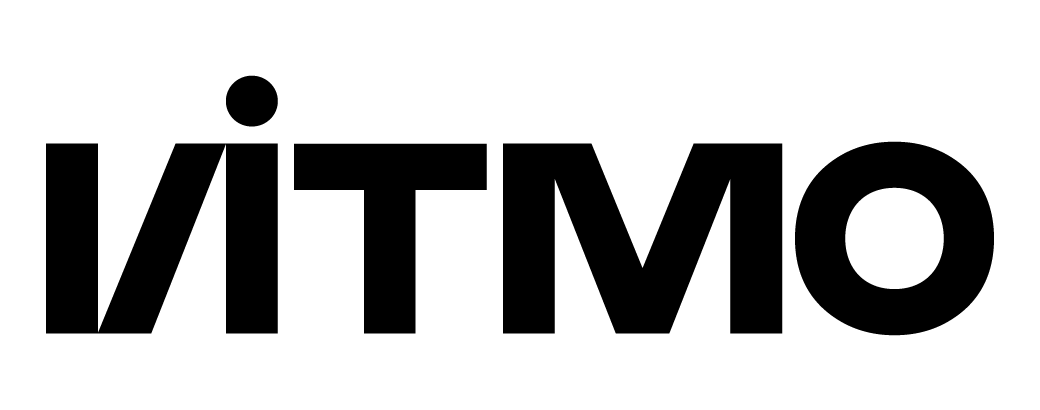
\includegraphics[width=3cm]{itmo_logo.png}
        % \\
        \city, \the\year\,
    \end{center}

\end{titlepage}

%<<<<<<<<<<<<<<<<< ТИТУЛЬНАЯ СТРАНИЦА <<<<<<<<<<<<<<<<<<<<<


%>>>>>>>>>>>>>>>>>>>>> СОДЕРЖАНИЕ >>>>>>>>>>>>>>>>>>>>>>>>>
% Содержание
    \tableofcontents
%<<<<<<<<<<<<<<<<<<<<< СОДЕРЖАНИЕ <<<<<<<<<<<<<<<<<<<<<<<<<


%%%%%%%%%%%%%%%%%%%%%%% КОД РАБОТЫ %%%%%%%%%%%%%%%%%%%%%%%%
%>>>>>>>>>>>>>>>>>>>'''''''''''''''''>>>>>>>>>>>>>>>>>>>>>
    \newpage
    % \Chapter{\lab\ \labnumber}{}{}

    \Section{Задание}

    \noindent
%    \textbf{
%    % Заглавное описание....:
%        Заголовок
%    }
%
%    \textit{
%    % Описание задания...
%        Описание
%    }

    \begin{enumerate}
        \setlength{\itemsep}{0pt} % Сокращение межстрочных расстояний
        \setlength{\parskip}{0pt}
        \setlength{\parsep}{0pt}
        \item Создать приведенное в варианте дерево каталогов и файлов с содержимым. В качестве корня дерева использовать каталог lab0 своего домашнего каталога. Для создания и навигации по дереву использовать команды: mkdir, echo, cat, touch, ls, pwd, cd, more, cp, rm, rmdir, mv.
           \begin{figure}[H] % 'H' -- вставить тут же (подключен модуль), обычный вариант: 'htpb'
							\centering
							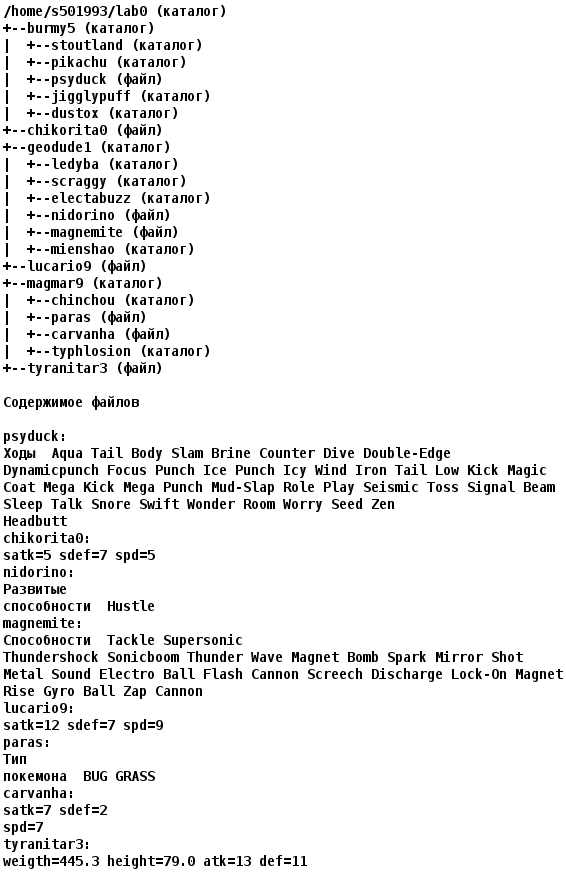
\includegraphics[width={\textwidth / 2}]{task1.png}
							\caption{Задание 1}
							\label{fig:enter-label}
					\end{figure}

				\item Установить согласно заданию права на файлы и каталоги при помощи команды chmod, используя различные способы указания прав.
        \begin{itemize}
            \setlength{\itemsep}{0pt} % Сокращение межстрочных расстояний
            \setlength{\parskip}{0pt}
            \setlength{\parsep}{0pt}
            \item burmy5: r-x--x-w-
            \item stoutland: -wxrw---x
            \item pikachu: владелец должен читать, записывать директорию и переходить в нее; группа-владелец должна читать и записывать директорию; остальные пользователи должны читать директорию
            \item psyduck: владелец должен читать файл; группа-владелец должна читать файл; остальные пользователи должны читать файл
            \item jigglypuff: права 700
            \item dustox: r-xrwxrwx
            \item chikorita0: ---rw--w-
            \item geodude1: владелец должен читать, записывать директорию и переходить в нее; группа-владелец должна читать директорию и переходить в нее; остальные пользователи должны записывать директорию
            \item ledyba: права 551
            \item scraggy: права 570
            \item electabuzz: владелец должен читать, записывать директорию и переходить в нее; группа-владелец должна читать директорию и переходить в нее; остальные пользователи должны записывать директорию
            \item nidorino: владелец должен читать и записывать файл; группа-владелец должна записывать файл; остальные пользователи должны записывать файл
            \item magnemite: владелец должен читать и записывать файл; группа-владелец должна не иметь никаких прав; остальные пользователи должны не иметь никаких прав
            \item mienshao: права 315
            \item lucario9: владелец должен не иметь никаких прав; группа-владелец должна читать файл; остальные пользователи должны читать и записывать файл
            \item magmar9: владелец должен записывать директорию и переходить в нее; группа-владелец должна читать, записывать директорию и переходить в нее; остальные пользователи должны читать директорию и переходить в нее
            \item chinchou: права 771
            \item paras: права 006
            \item carvanha: rw--w-r--
            \item typhlosion: права 551
            \item tyranitar3: владелец должен читать и записывать файл; группа-владелец должна записывать файл; остальные пользователи должны не иметь никаких прав
        \end{itemize}

				\item Скопировать часть дерева и создать ссылки внутри дерева согласно заданию при помощи команд cp и ln, а также комманды cat и перенаправления ввода-вывода.
				\begin{itemize}
					\item скопировать файл tyranitar3 в директорию lab0/magmar9/typhlosion
					\item создать символическую ссылку c именем Copy\_2 на директорию burmy5 в каталоге lab0
					\item cоздать жесткую ссылку для файла chikorita0 с именем lab0/burmy5/psyduckchikorita
					\item скопировать рекурсивно директорию burmy5 в директорию lab0/geodude1/scraggy
					\item объединить содержимое файлов lab0/magmar9/carvanha, lab0/geodude1/nidorino, в новый файл lab0/chikorita0\_17
					\item cоздать символическую ссылку для файла chikorita0 с именем lab0/burmy5/psyduckchikorita
					\item скопировать содержимое файла lucario9 в новый файл lab0/magmar9/paraslucario
				\end{itemize}

				\item Используя команды cat, wc, ls, head, tail, echo, sort, grep выполнить в соответствии с вариантом задания поиск и фильтрацию файлов, каталогов и содержащихся в них данных.
				\begin{itemize}
					\item Рекурсивно подсчитать количество строк содержимого файлов из директории lab0, имя которых заканчивается на 'o', результат записать в файл в директории /tmp, подавить вывод ошибок доступа
					\item Вывести четыре последних элемента рекурсивного списка имен и атрибутов файлов в директории lab0, содержащих строку "du", список отсортировать по возрастанию даты изменения записи о файле, добавить вывод ошибок доступа в стандартный поток вывода
					\item Рекурсивно вывести содержимое файлов из директории lab0, имя которых заканчивается на 'u', строки отсортировать по имени a->z, ошибки доступа не подавлять и не перенаправлять
					\item Вывести рекурсивно список имен и атрибутов файлов в директории lab0, содержащих строку "ca", список отсортировать по возрастанию размера, ошибки доступа перенаправить в файл в директории /tmp
					\item Вывести три первых элемента рекурсивного списка имен и атрибутов файлов в директории lab0, список отсортировать по возрастанию даты изменения записи о файле, ошибки доступа перенаправить в файл в директории /tmp
					\item Рекурсивно подсчитать количество символов содержимого файлов из директории lab0, имя которых начинается на 'p', отсортировать вывод по увеличению количества, ошибки доступа не подавлять и не перенаправлять
				\end{itemize}

				\item Выполнить удаление файлов и каталогов при помощи команд rm и rmdir согласно варианту задания.
				\begin{itemize}
					\item Удалить файл tyranitar3
					\item Удалить файл lab0/magmar9/carvanha
					\item удалить символические ссылки Copy*
					\item удалить жесткие ссылки lab0/burmy5/psyduckchikori*
					\item Удалить директорию burmy5
					\item Удалить директорию lab0/geodude1/mienshao
				\end{itemize}
    \end{enumerate}


    \newpage
    \Section{Ход работы}
    Для удобства запуска и проверки задание выполнено с помощью \verb|bash| скрипта \ref{lst:bash}, содержащего необходимый набор команд, который запускается непосредственно на сервере.
    \lstinputlisting[caption={Исходный код программы},label={lst:bash},language=Java]{../src/lab1.sh}

% Выполнение задания...
    \newpage

    \Section{Вывод}
        В процессе выполнения лабораторной работы по информатике я вспомнил методы перевода чисел между различными системами счисления \cite{1}, а также ознакомился и научился работать с незнакомыми мне раннее системами счисления Бергмана, фибоначчиевой и факториальной \cite{2}.
    \newpage
%<<<<<<<<<<<<<<<<<<<<<< КОД РАБОТЫ <<<<<<<<<<<<<<<<<<<<<<<<


%>>>>>>>>>>>>>>>> СПИСОК ЛИТЕРАТУРЫ >>>>>>>>>>>>>>>>>>>>>>>
    \begin{thebibliography}{}
    \bibitem{1}Орлов С. А., Цилькер Б. Я. Организация ЭВМ и систем: Учебник для вузов. 2-е изд. – СПб.: Питер, 2011. – 688 с.: ил., Приложение А «Арифметические основы вычислительных машин». URL: \url{https://bit.ly/4dzgo3u} (Дата обращения: 10.09.25) \\
    \bibitem{2}Алексеев Е.Г., Богатырев С.Д. Информатика. Мультимедийный электронный учебник. Раздел 3 «Системы счисления». URL: \url{http://inf.e-alekseev.ru/text/Schisl.html} (Дата обращения: 10.09.25)
\end{thebibliography}  % Для соответсвия гост, придется доработать. Нужен файл .bib
%<<<<<<<<<<<<<<<<<<<< СПИСОК ЛИТЕРАТУРЫ <<<<<<<<<<<<<<<<<<<

    % \Section{Список использованных источников}
    % \begin{thebibliography}{}
    %     \bibitem{1}Орлов С. А., Цилькер Б. Я. Организация ЭВМ и систем: Учебник для вузов. 2-е изд. – СПб.: Питер, 2011. – 688 с.: ил., Приложение А «Арифметические основы вычислительных машин». URL: \url{https://bit.ly/4dzgo3u} (Дата обращения: 10.09.25) \\
    %     \bibitem{2}Алексеев Е.Г., Богатырев С.Д. Информатика. Мультимедийный электронный учебник. Раздел 3 «Системы счисления». URL: \url{http://inf.e-alekseev.ru/text/Schisl.html} (Дата обращения: 10.09.25)
    % \end{thebibliography}
    \end{document}
%<<<<<<<<<<<<<<<< ,,,,,,,,,,,,,,,,,,,,,,, <<<<<<<<<<<<<<<<<
%<<<<<<<<<<<<<<<<<<< СОДЕРЖИМОЕ ОТЧЕТА <<<<<<<<<<<<<<<<<<<<